% Nominal single-target comparison on N(2.2,2.2,pi/2).
% Values match Table~\ref{tab:single_target_nominal_comparison}: the Adam bars are the
% best NOMINAL solution (T = 70 ns), not the 60 ns plan selected by the noisy objective.
%   Adam  (70 ns) : C=0.1576  F=0.99662  L=2.82e-4  T=70
%   TRPO nominal  : C=0.2982  F=0.99415  L=1.60e-3  T=116
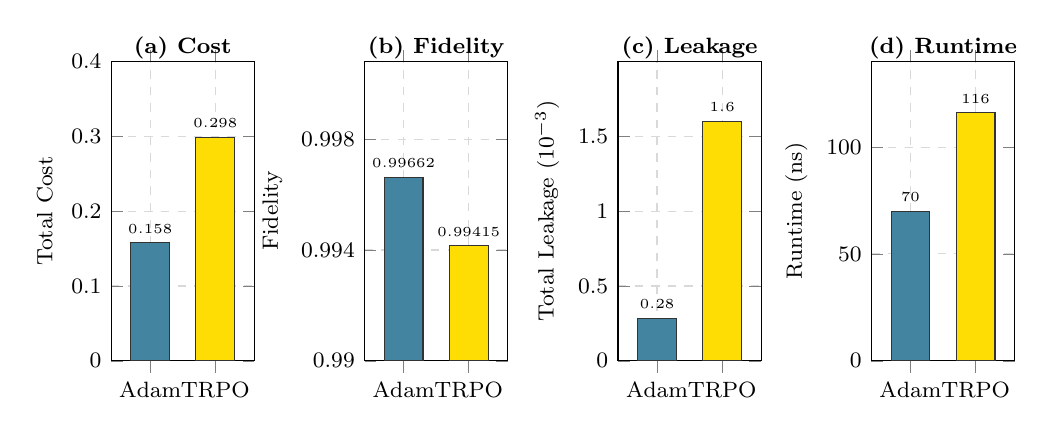
\begin{tikzpicture}
    \pgfplotsset{
        every axis/.append style={
            scale only axis,
            height=3.8cm,
            width=0.15\linewidth,
            grid=major,
            grid style={dashed, gray!30},
            ybar,
            bar width=14pt,
            enlarge x limits=0.6,
            symbolic x coords={Adam, TRPO},
            xtick={Adam, TRPO},
            x tick label style={font=\footnotesize},
            tick label style={font=\footnotesize},
            label style={font=\footnotesize},
            title style={font=\footnotesize\bfseries, yshift=-1ex},
            nodes near coords,
            nodes near coords align={vertical},
            every node near coord/.append style={font=\tiny},
        }
    }

    % Panel (a): Total cost
    \begin{axis}[
        name=plot_cost,
        ylabel={Total Cost},
        title={(a) Cost},
        ymin=0, ymax=0.40,
        every node near coord/.append style={/pgf/number format/fixed, /pgf/number format/precision=3},
    ]
    \addplot[fill=cyan!60!black, draw=black!80, bar shift=0pt] coordinates {(Adam, 0.1576)};
    \addplot[fill=yellow!80!orange, draw=black!80, bar shift=0pt] coordinates {(TRPO, 0.2982)};
    \end{axis}

    % Panel (b): Nominal fidelity
    \begin{axis}[
        name=plot_fid,
        at={(plot_cost.south east)},
        anchor=south west,
        xshift=1.4cm,
        ylabel={Fidelity},
        title={(b) Fidelity},
        ymin=0.990, ymax=1.0008,
        ytick={0.990, 0.994, 0.998},
        yticklabel style={/pgf/number format/fixed, /pgf/number format/precision=3},
        every node near coord/.append style={/pgf/number format/fixed, /pgf/number format/precision=5},
    ]
    \addplot[fill=cyan!60!black, draw=black!80, bar shift=0pt] coordinates {(Adam, 0.99662)};
    \addplot[fill=yellow!80!orange, draw=black!80, bar shift=0pt] coordinates {(TRPO, 0.99415)};
    \end{axis}

    % Panel (c): Total leakage, linear axis in units of 1e-3
    % (a log axis cannot be used with ybar: the bars would be drawn from y=0, i.e. -infinity)
    \begin{axis}[
        name=plot_leak,
        at={(plot_fid.south east)},
        anchor=south west,
        xshift=1.4cm,
        ylabel={Total Leakage ($10^{-3}$)},
        title={(c) Leakage},
        ymin=0, ymax=2.0,
        ytick={0, 0.5, 1.0, 1.5},
        yticklabel style={/pgf/number format/fixed, /pgf/number format/precision=1},
        nodes near coords={\pgfmathprintnumber[fixed,precision=2]{\pgfplotspointmeta}},
    ]
    \addplot[fill=cyan!60!black, draw=black!80, bar shift=0pt] coordinates {(Adam, 0.282)};
    \addplot[fill=yellow!80!orange, draw=black!80, bar shift=0pt] coordinates {(TRPO, 1.600)};
    \end{axis}

    % Panel (d): Effective runtime
    \begin{axis}[
        name=plot_time,
        at={(plot_leak.south east)},
        anchor=south west,
        xshift=1.4cm,
        ylabel={Runtime (ns)},
        title={(d) Runtime},
        ymin=0, ymax=140,
        nodes near coords={\pgfmathprintnumber[fixed,precision=0]{\pgfplotspointmeta}},
    ]
    \addplot[fill=cyan!60!black, draw=black!80, bar shift=0pt] coordinates {(Adam, 70.0)};
    \addplot[fill=yellow!80!orange, draw=black!80, bar shift=0pt] coordinates {(TRPO, 116.0)};
    \end{axis}

\end{tikzpicture}
